\begin{frame}{Proposta}
    \begin{enumerate}
        \item Trabalhos relacionados.
        \item Algoritmos.
        \begin{itemize}
            \item Algoritmos Determinísticos.
            \item Arquiteturas Paralelas.
        \end{itemize}
        \item Cenário de execução.
        \item Técnicas e ferramentas.
        \item Cenário de teste.
    \end{enumerate}
\end{frame}

\begin{frame}{Algoritmos Determinísticos}
    Algoritmos Determinísticos:

    \begin{itemize}
        \item Resultados consistentes para determinada entrada.
        \item Previsíveis.
        \item Garantia de solução ótima.
        \item Características essenciais para garantir confiabilidade no sistema.
    \end{itemize}
\end{frame}

\begin{frame}{Arquiteturas Paralelas}
    Arquiteturas Paralelas:

    \begin{itemize}
        \item \textit{SIMD} e \textit{MIMD}.
        \item Otimizar a execução de operações em grandes volumes de dados.
        \item Alto desempenho.
    \end{itemize}
\end{frame}

\begin{frame}{Trabalhos Relacionados}
    \begin{figure}
        \centering
        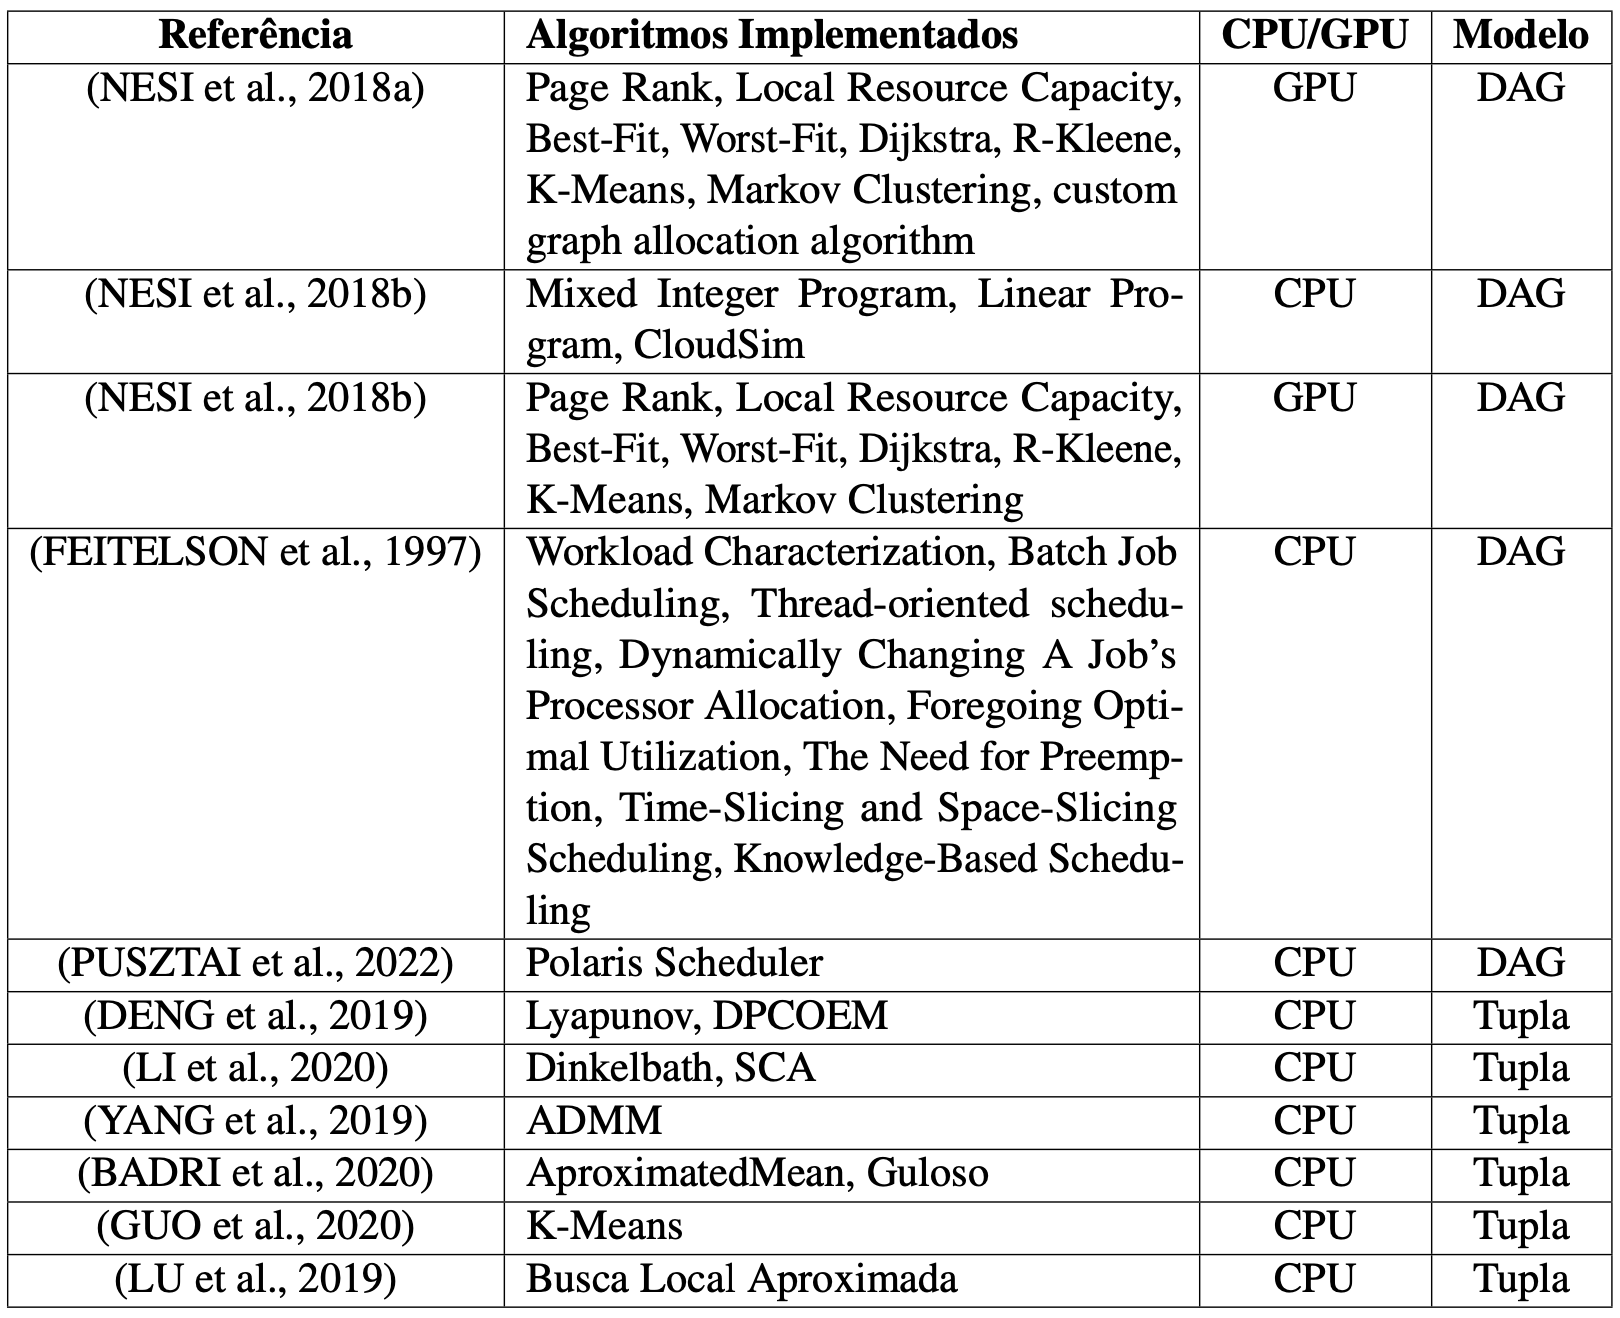
\includegraphics[width=0.9\textwidth]{Figuras/trabalhos-relacionados.png}
    \end{figure}
\end{frame}

\begin{frame}{Algoritmos}
    \begin{table}[ht]
        \centering
        \scriptsize
        \begin{tabular}{|c|c|c|c|}
            \hline
            \textbf{Algoritmo} & \textbf{Categoria} & \textbf{Complexidade} & \textbf{CPU/GPU} \\
            \hline
            Prefix Sum & DP & $O(n)$ & GPU \\
            \hline
            Busca Binária & Busca & $O(\log n)$ & CPU \\
            \hline
            Merge Sort & Ordenação & $O(n \log n)$ & CPU \\
            \hline
            Topological Sort & Ordenação & $O(V + E)$ & CPU \\
            \hline
            Radix Sort & Ordenação & $O(nw)$ & GPU \\
            \hline
            K-means & Agrupamento & $O(nkdi)$ & GPU \\
            \hline
            DBSCAN & Agrupamento & $O(n^2)$ & GPU \\
            \hline
            Hierarchical Clustering & Agrupamento & $O(n^3)$ & CPU \\
            \hline
            Markov Clustering & Agrupamento & $O(n^3)$ & GPU \\
            \hline
            PageRank & Ranqueamento & $O(n + m)$ & GPU \\
            \hline
            Dijkstra & Menor Caminho & $O(E + V \log V)$ & CPU \\
            \hline
            Floyd-Warshall & Menor Caminho & $O(n^3)$ & CPU \\
            \hline
            A* & Menor Caminho & $O(E \log V)$ & CPU \\
            \hline
            Kruskal & MST & $O(E \log E)$ & CPU \\
            \hline
            Prim & MST & $O(E + V \log V)$ & CPU \\
            \hline
            Edmonds-Karp & Fluxo & $O(VE^2)$ & CPU \\
            \hline
            Min-Cost Max-Flow & Fluxo & $O(V^2E^2)$ & CPU \\
            \hline
            Dinic & Fluxo & $O(V^2E)$ & CPU \\
            \hline
            Gaussian Elimination & Otimização & $O(n^3)$ & GPU \\
            \hline
            Hungarian & Otimização & $O(n^3)$ & CPU \\
            \hline
        \end{tabular}
        \caption{Algoritmos presentes no \textit{framework} proposto.}
        \label{table:algorithms}
    \end{table}
\end{frame}

% talvez remover esse slide
\begin{frame}{Cenário de execução}
    \begin{figure}
        \centering
        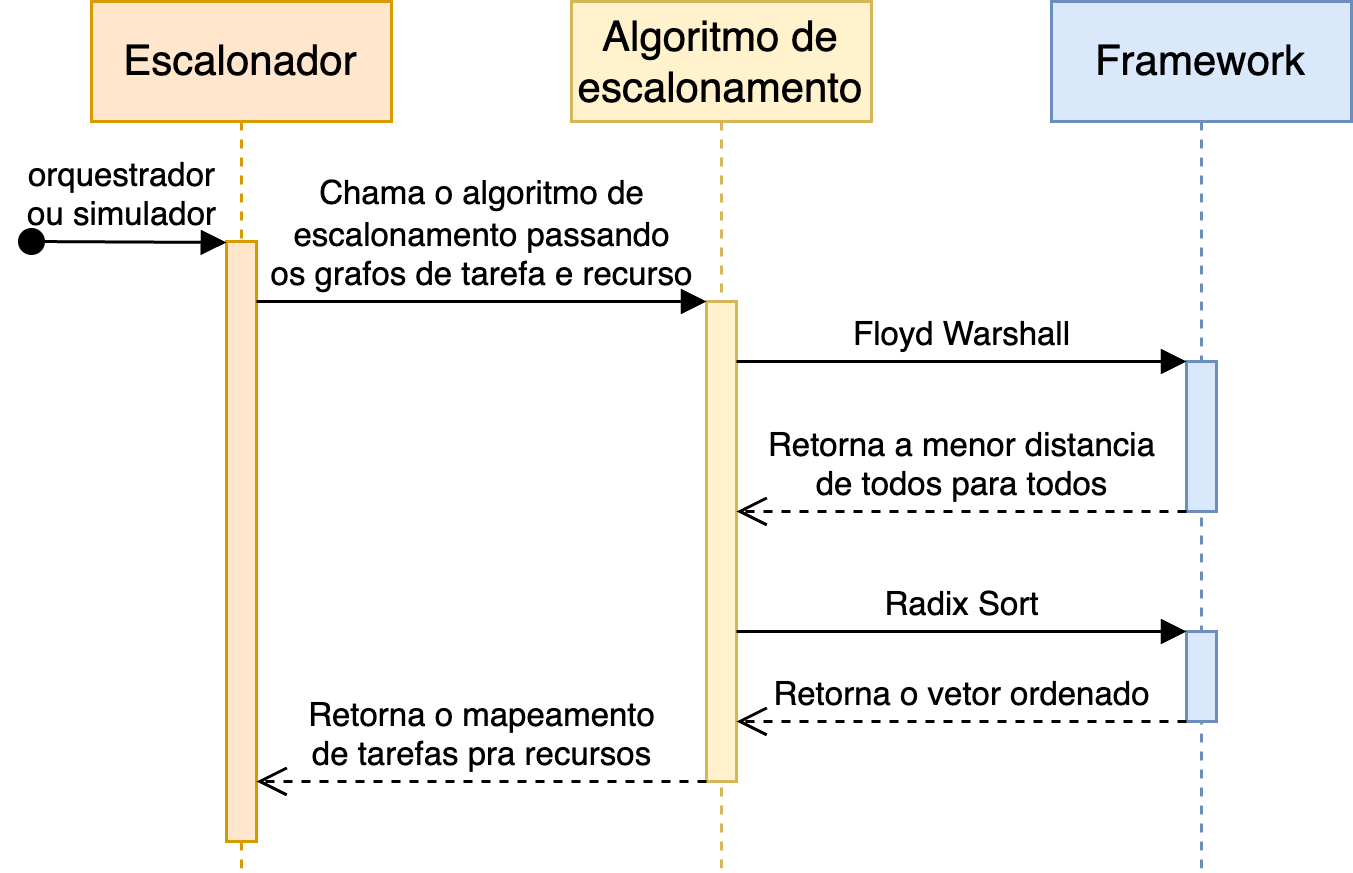
\includegraphics[width=\textwidth]{Figuras/framework-usage-2.png}
    \end{figure}
\end{frame}

\begin{frame}{Código Exemplo}
    \begin{figure}
        \centering
        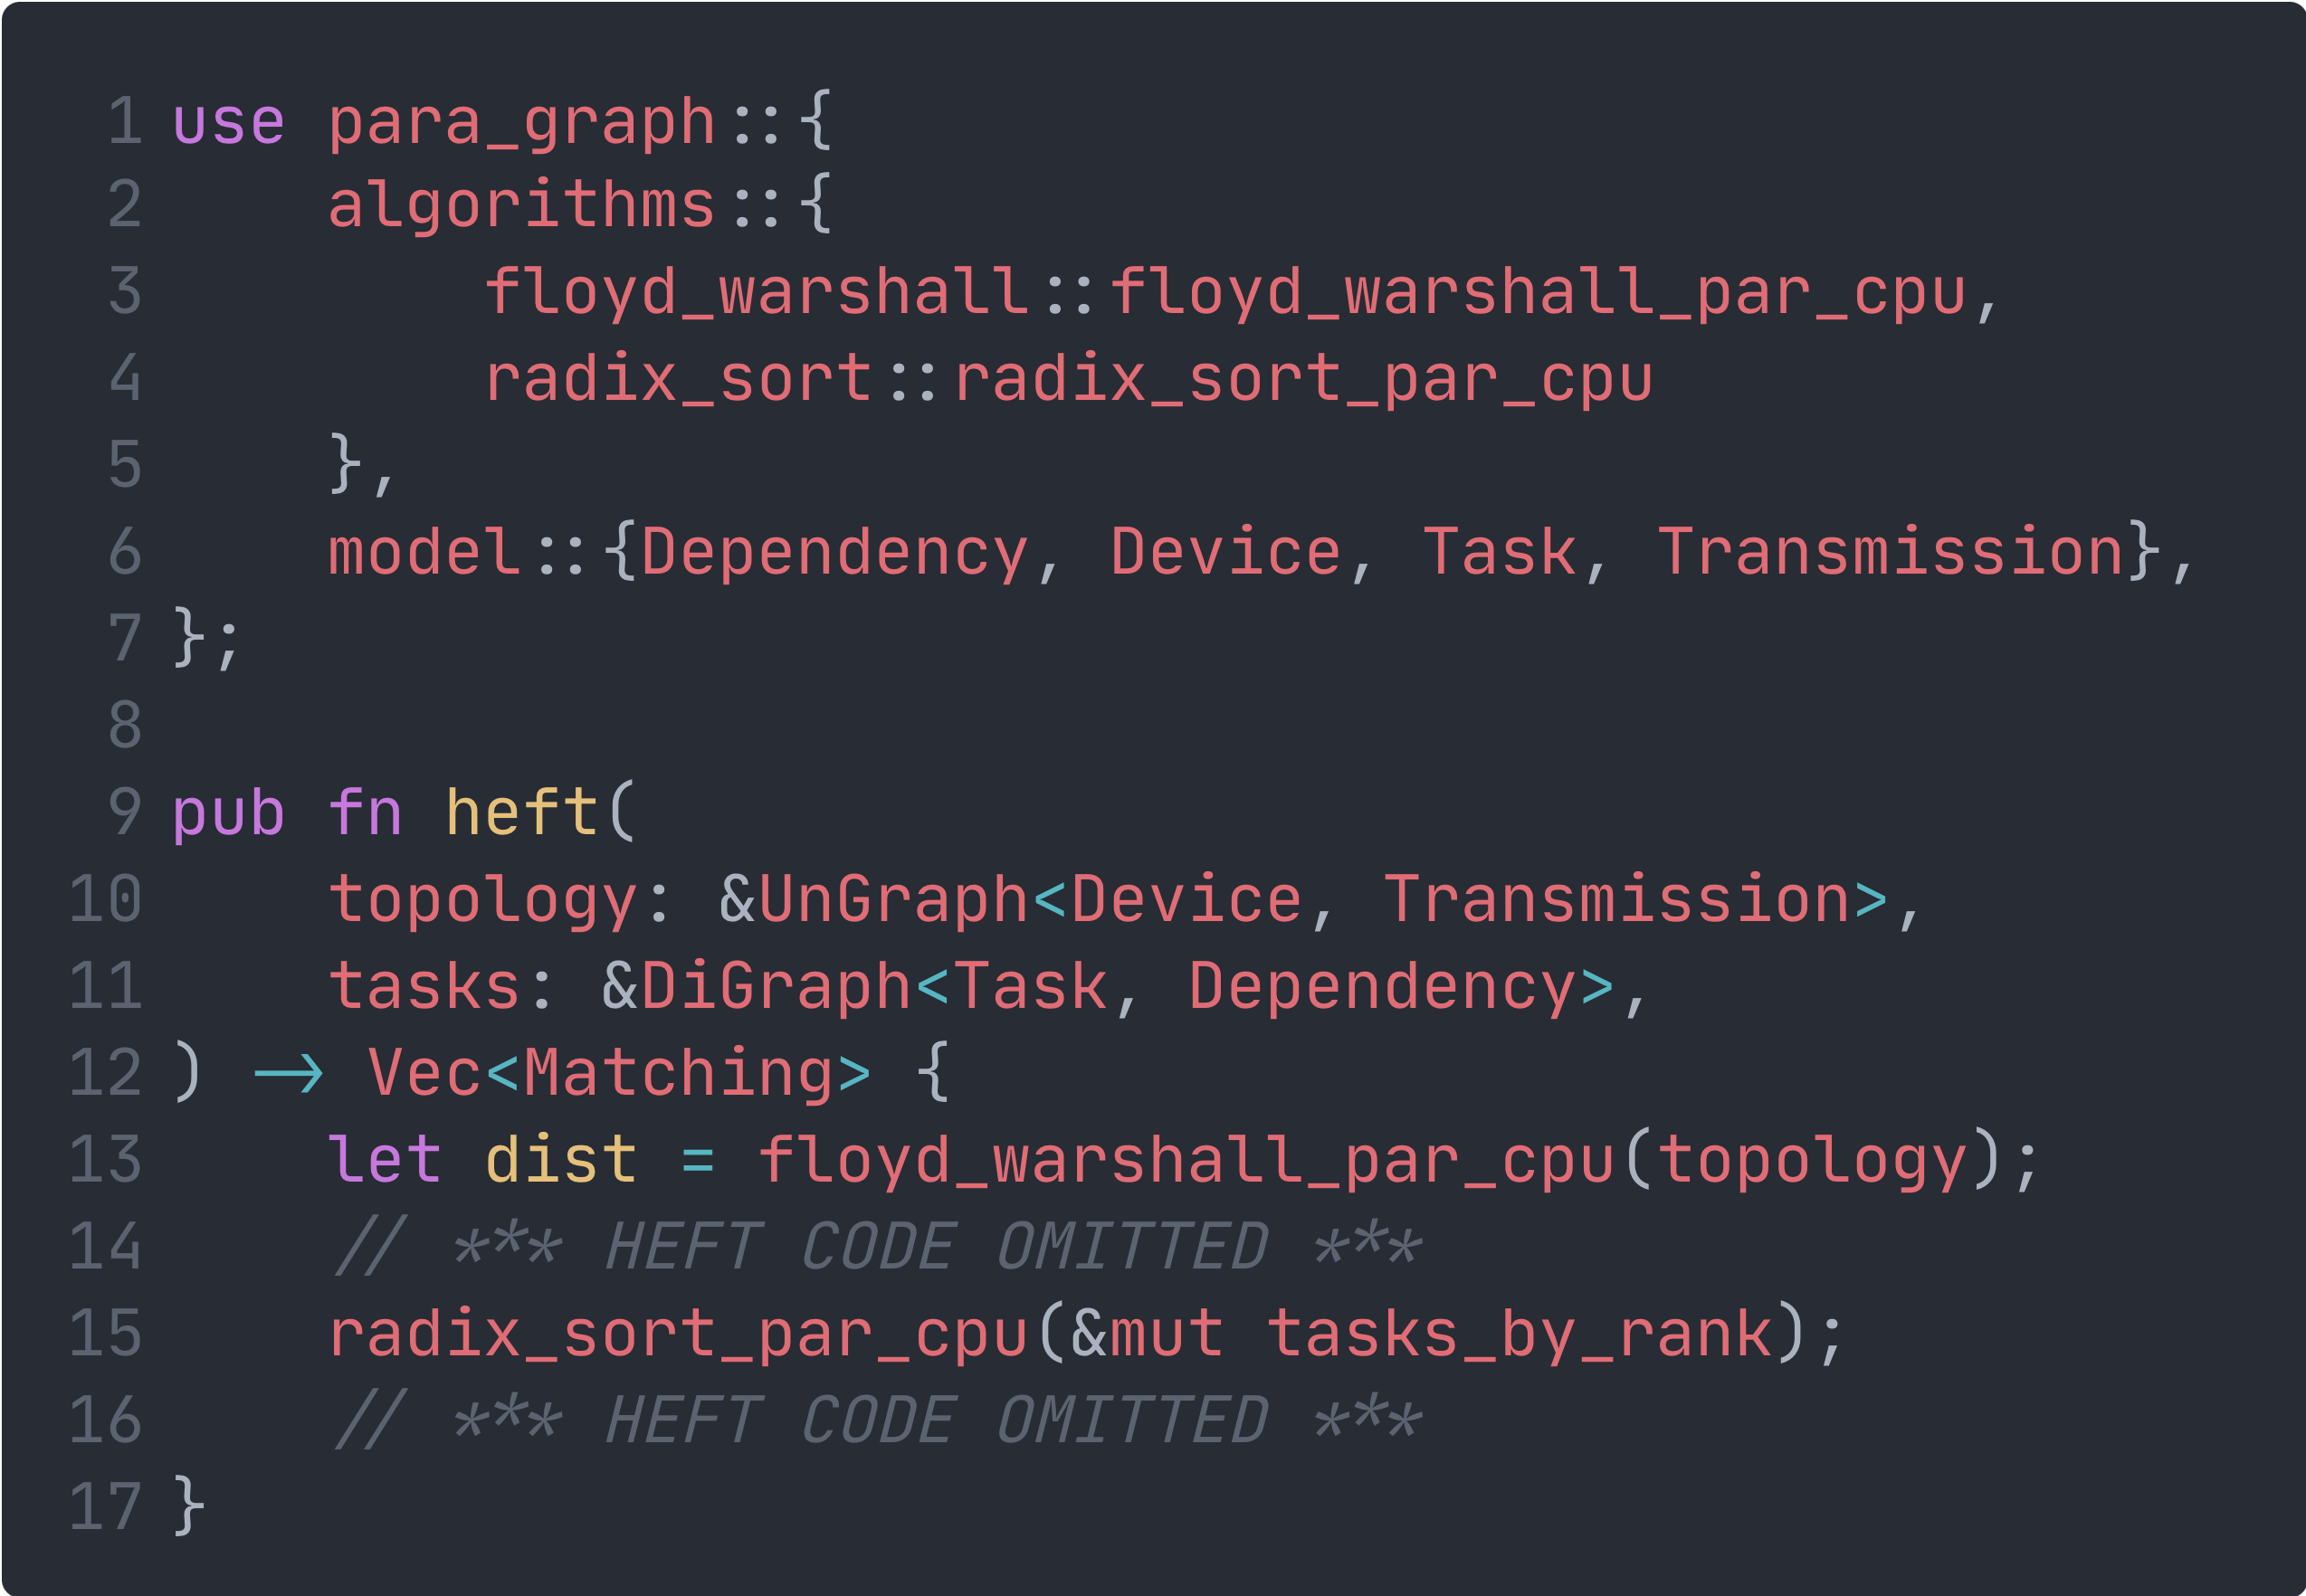
\includegraphics[width=\textwidth]{Figuras/code-2.png}
    \end{figure}
\end{frame}

\begin{frame}{Técnicas e Ferramentas}
    \begin{columns}
    \begin{column}{0.9\textwidth}
    Rust:
    \begin{itemize}
        \item[--] Linguagem moderna.
        \item[--] Segurança de memória.
        \item[--] Alto desempenho. 
        \item[--] \textit{Petgraph}.
        \item[--] \textit{Fearless Concurrency}.
        \item[--] \textit{Rayon}.
    \end{itemize}
    \end{column}

    \begin{column}{0.1\textwidth}
        \begin{figure}
            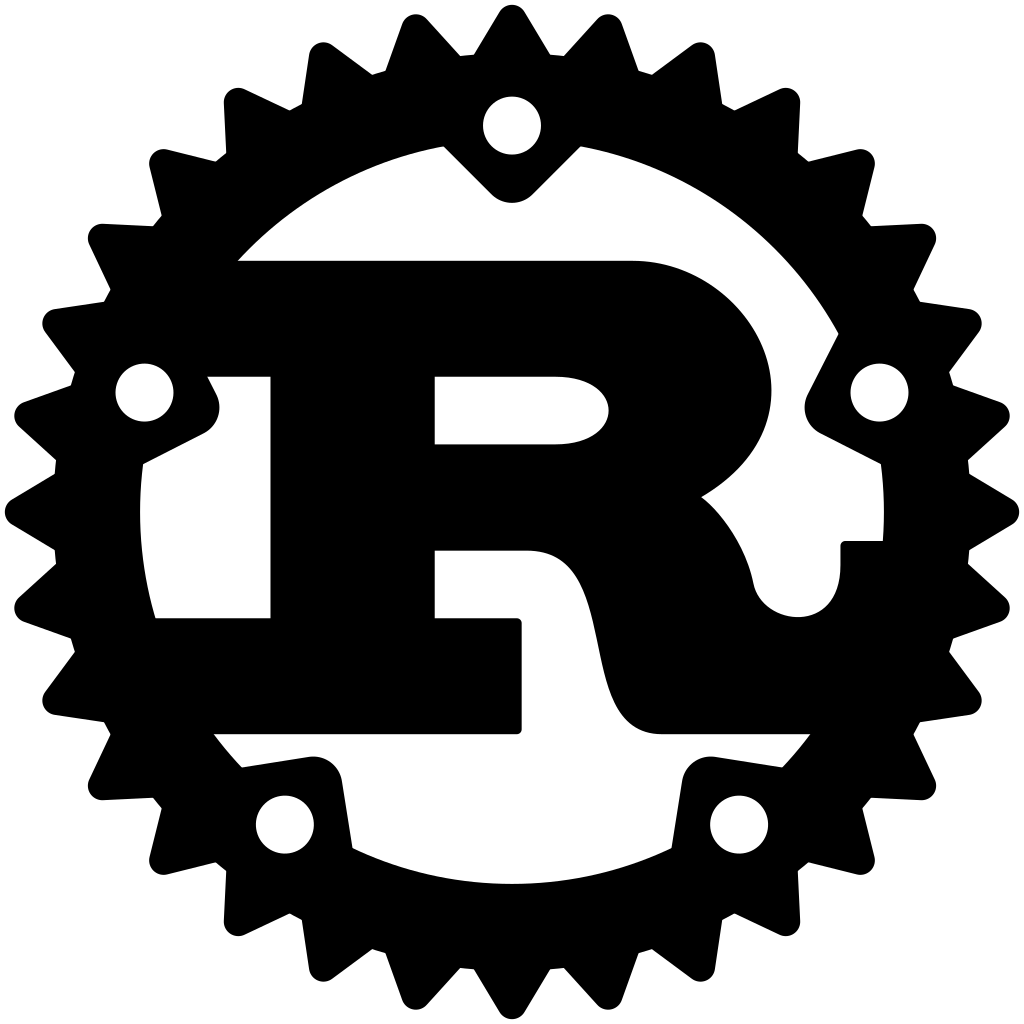
\includegraphics[width=\textwidth]{Figuras/Rust Logo.svg.png}
        \end{figure}
    \end{column}
    \end{columns}
\end{frame}

% \begin{frame}{Fearless Concurrency}
%     \begin{figure}
%         \centering
%         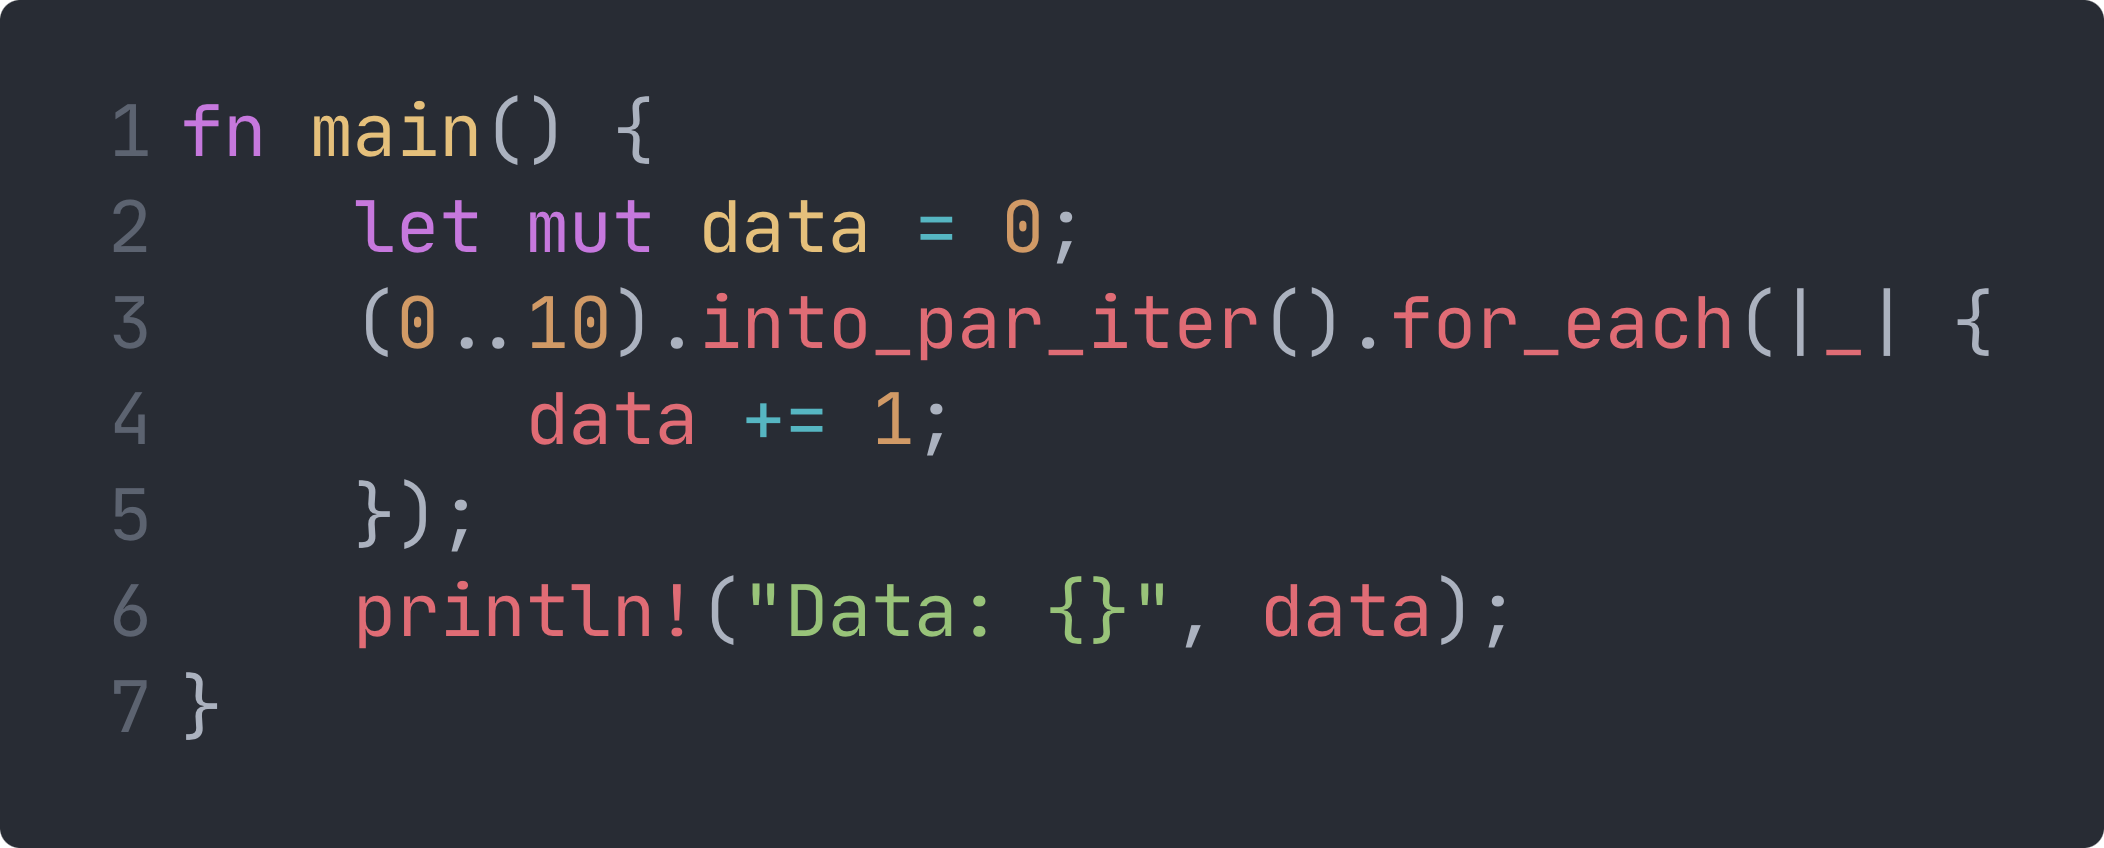
\includegraphics[width=\textwidth]{Figuras/fearlessconcurrency.png}
%     \end{figure}
% \end{frame}

\begin{frame}{Técnicas e Ferramentas}
    \begin{columns}
    \begin{column}{0.9\textwidth}
    C++:
    \begin{itemize}
        \item[--] Excelente suporte a \textit{GPUs}.
        \item[--] \textit{OpenAcc}.
        \item[--] Comunicação por meio de \textit{Foreign Function Interface}.
    \end{itemize}
    \end{column}

    \begin{column}{0.1\textwidth}
        \begin{figure}
            
\includegraphics[width=\textwidth]{Figuras/C++ Logo.png}
        \end{figure}
    \end{column}
    \end{columns}
\end{frame}

\begin{frame}{Cenário experimental}
    Métricas:
    \begin{itemize}
        \item[--] Speedup, Eficiência, Escalabilidade, Overhead.
    \end{itemize}

    \vspace{1em}

    % Base de dados aberta:
    % \begin{itemize}
    %     \item[--] \textit{Politecnico di Milano}.
    %     \item[--] Dados reais e sintéticos.
    %     \item[--] Grafos de diversos tamanhos e formatos.
    % \end{itemize}

    \vspace{1em}

    Infraestrutura local do LabP2D:
    \begin{itemize}
        \item[--] 2 CPUs Intel Xeon Silver 2.2GHz.
        \item[--] NVIDIA RTX 3090 24GB.
    \end{itemize}
\end{frame}
